\chapter{Design of MPI\_T support in Caliper}

Caliper is an application introspection tool that relies on source code annotations to collect information and perform profiling related tasks. I shall first provide a basic overview of relevant Caliper concepts before describing the MPI\_T support in Caliper. 

\section{Caliper Concepts}
\subsection{Caliper API}
Caliper provides an application level API that acts as the portal for carrying out performance measurements. Caliper also provides high-level annotation macros that are user-friendly. The basic idea behind the source-code annotation API is to associate performance measurements with user-defined, high-level \textit{context information}. These source code annotations act as hooks for background processing. Caliper is built into a library and linked into the application. Figure \ref{fig:caliexample}\footnote{Image taken from: https://llnl.github.io/Caliper} is an example of a Caliper-annotated \verb+C+\texttt{++} source code.
\subsection{Attributes: Caliper's Building Blocks}
Caliper provides a generic \textit{key-value} data model for storing performance data of all kinds. Caliper \textit{attributes} are the basic elements of the Caliper data model. The keys need to have a unique name and a type. They can also optionally have properties which determine how the attributes get processed. An example would be an attribute to track PAPI counters or an attribute to track the total time spent inside a routine or code section. 
\par Among all the properties that an attribute can have, the most important property in the context of MPI\_T is the \verb+AS_VALUE+ property. Attributes with the \verb+AS_VALUE+ property set to true cannot be nested. For example, the attribute to track PAPI counters cannot be nested, but the attribute to track the time spent inside a routine is nested.
\begin{center}
	\begin{figure*}[tbp!]
         \centering
  \captionsetup{justification=centering}
		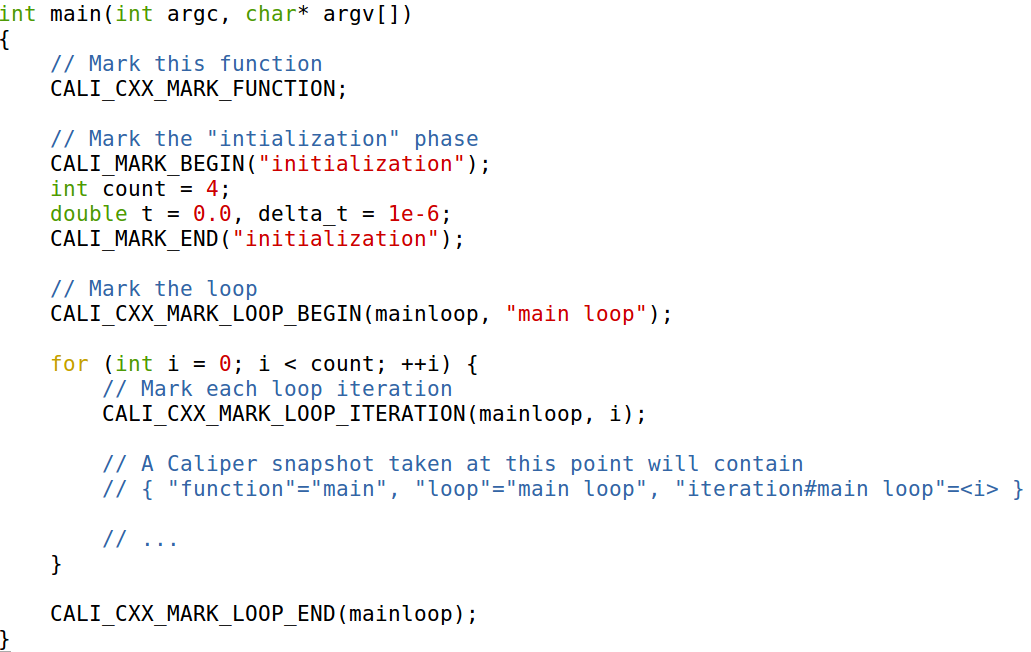
\includegraphics[scale=0.3, width=\columnwidth, keepaspectratio]{figures/cali-example}
		\caption{Caliper annotated source code}
		\label{fig:caliexample}
	\end{figure*}
\end{center}

\subsection{Blackboards and Snapshots}
Whenever a performance measurement is made by use of Caliper's measurement API, the values of one or more attributes are updated in an internal data-structure referred to as the \textit{blackboard}. This blackboard is a runtime buffer that is used to combine active attributes, and is updated by Caliper data providers (annotations).
\par A \textit{snapshot} saves the current context of the blackboard. A snapshot can be triggered independently of blackboard updates. Additional information can be added to the snapshot via callbacks to snapshot events. 
\subsection{Services}
Caliper \emph{services} are the basic building blocks that can be combined freely to realize advanced profiling/tracing capabilities. Services are essentially plugins that register callbacks for events of interest. During Caliper initialization, the registered initialization function of each required service is invoked, and the service then performs start-up related tasks inside this initialization function. 
\par An example of a service is the \textit{MPI} service. The MPI service keeps track of the time spent inside MPI calls by utilizing the PMPI interface. The \textit{recorder} service writes Caliper snapshot records into a file using a custom text-based I/O format. The recorder service in conjunction with the MPI service can be used to gather a basic profile of an MPI application. Figure \ref{fig:caliservices} is an illustration of this use case. 
\begin{center}
	\begin{figure*}[bp!]
         \centering
  \captionsetup{justification=centering}
		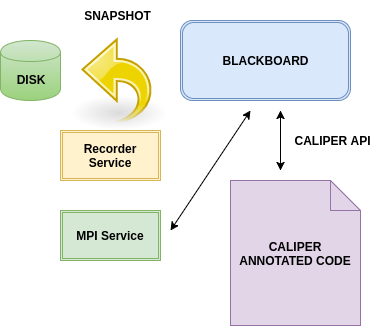
\includegraphics[scale=0.7, keepaspectratio]{figures/cali-services}
		\caption{MPI profiling: Caliper service flow}
		\label{fig:caliservices}
	\end{figure*}
\end{center}

\section {MPI\_T Service: Supporting Performance Introspection}
This section describes the design of the MPI\_T service that performs runtime MPI library introspection through the MPI\_T interface. As of the time being, this service does not support performance monitoring or tuning through the MPI\_T interface. 
\section{Service Registration}
During the registration phase for the MPI\_T service, the MPI\_T performance session is created. The handles for all the PVARs exported at the time of service registration are allocated. It is important to note that service registration may happen before \verb+MPI_Init+ is invoked. If this is the case, the number of PVARs exported may be zero. The design should account for this scenario.
\par In the next section, I shall discuss the complexities that arise with allocating handles for PVARs in detail, and how the design addresses these issues.
\section{PVAR Handle Allocation}
Before a tool can read the value of a PVAR, it must first allocate a \emph{handle} for the PVAR. The MPI\_T interface specifies a function that allows a tool to know the number of PVARs exported by an MPI implementation at any given point in time. Recall that the number of PVARs exported can dynamically increase, and that PVARs can be bound to MPI objects. Like TAU, Caliper only supports PVARs that are exported immediately after \verb+MPI_Init+ by invoking the handle allocation routine inside the PMPI wrapper for \verb+MPI_Init+. Any increase in the number of PVARs after this point is ignored by Caliper. 
\par PVARs can be bound to MPI objects, and such PVARs can provide fine-grained detail about MPI. For example, a PVAR representing the number of messages sent can potentially be bound to an MPI communicator object. This way, it would be possible for a tool to distinguish the quantity of communication across communicators/process groups instead of presenting an aggregated view to the user.
\par Handles for PVARs not bound to any object (\verb+MPI_T_BIND_NO_OBJECT+) can be allocated at any time --- specifically, this is done inside the registration phase for the MPI\_T service, and inside the PMPI wrapper for \verb+MPI_Init+. In order to allocate handles for PVARs bound to MPI objects, we need a reference (address) to the MPI object in question. The ideal location for the MPI\_T service to grab these references would be during MPI object creation. Briefly, the following steps are necessary to allocate such handles:
\begin{itemize}
\item Identify the corresponding MPI object creation routine for the object in question
\item Intercept the object creation routine (through PMPI)
\item Allocate handles for all PVARs bound to the given object type
\end{itemize}
It is possible that multiple handles are associated with a PVAR bound to an MPI object --- one for each such MPI object created. The supported MPI object types in MPI\_T and their corresponding object routines used to allocate handles are presented in Table \ref{tab:caliperhandles}.
\begin{table*}[!htbp]
  \centering
  \small
  \captionsetup{justification=centering}
  \caption{Caliper: PVAR handle allocation routines for supported MPI object types}
  \label{tab:caliperhandles}
  \resizebox{0.65\columnwidth}{!}{\begin{tabular}{|c|l|}
    \toprule
    MPI Object Type&MPI Object Creation Routine\\
     \midrule
     MPI Communicator&MPI\_Comm\_Create\\
     MPI Error Handler&MPI\_Err\_handler\\
     MPI File&MPI\_File\_open\\
     MPI Groups&MPI\_Group\_create\\
     MPI Reduction Operators&MPI\_Op\_create\\
     MPI Info Objects&MPI\_Info\_create\\
     MPI Window Objects&MPI\_Win\_create\\
     MPI Datatypes&\textit{Not Supported}\\
     MPI Message Objects&\textit{Not Supported}\\
     MPI Request Objects&\textit{Not Supported}\\
  \bottomrule
\end{tabular}}
\end{table*}

\section{PVAR Classes and Notion of Aggregability}
Depending on what they represent, PVARs are categorized by the MPI standard into counters, state variables, watermarks, etc., and are handled differently by Caliper. We define the notion of \textit{aggregatability} as follows: Any PVAR on which it is \emph{meaningful} to apply one or more of the operators --- SUM, MAX, MIN, AVG, COUNT is defined as aggregatable.
\par Along with other information, a call to \verb+MPIT_pvar_get_info+ returns the \emph{CLASS} to which the PVAR belongs. Below we describe the various PVAR classes supported by the MPI standard and how each class is handled by Caliper:
\begin{itemize}
	\item \verb+MPI_T_PVAR_CLASS_TIMER+, \verb+MPI_T_PVAR_CLASS_AGGREGATE+, \verb+MPI_T_PVAR_CLASS_COUNTERS+: These are free-counting, monotonically increasing values. As such, they are not aggregatable, but by storing the previous value for these counters and timers, the difference between the current and previous value is a derived metric that is aggregatable by use of \emph{SUM}, \emph{MAX}, \emph{MIN}, \emph{AVG} operators. Storing this difference is more useful than just the raw counter values, as one would typically be interested in the \emph{change} caused to any of these PVARs rather than the raw value itself.
	\item \verb+MPI_T_PVAR_CLASS_STATE+: Represents MPI state at any instant in time. Non-aggregatable value.
	\item \verb+MPI_T_PVAR_CLASS_SIZE+: Represents size of an MPI resource. Non-aggregatable value.
	\item \verb+MPI_T_PVAR_CLASS_LEVEL+, \verb+MPI_T_PVAR_CLASS_PERCENTAGE+: Represents the instantaneous level or percentage utilization of an MPI resource. It is meaningful to apply the \emph{AVG}, \emph{MIN}, \emph{MAX} operators, and hence these classes are aggregatable.
	\item \verb+MPI_T_PVAR_CLASS_HIGHWATERMARK+, \verb+MPI_T_PVAR_CLASS_LOWWATERMARK+: As such, these classes are non-aggregatable. However, one can define aggregatable derived metrics out of these PVARs. Specifically, Caliper defines two derived metrics --- A boolean that tells us if the watermark has gone up from the last time it was read, and a double value specifying the \emph{change} in the value between successive reads. Both of these derived metrics are aggregatable quantities as one can apply the \emph{COUNT} and/or \emph{SUM} operator to them.
	\item \verb+MPI_T_PVAR_CLASS_GENERIC+: PVARs that do not fall into any of the above classes. These PVARs would need to be handled on a case-by-case basis, and thus, for now, we define these to be non-aggregatable.
\end{itemize}

\section{Creating Caliper Attributes for PVARs}
The basic data unit in Caliper is an attribute. An attribute is a key-value pair that has certain properties. For each PVAR exposed by the MPI library, Caliper defines an attribute with the same name as the PVAR. Each PVAR attribute has the following properties:
\begin{itemize}
	\item \verb+CALI_ATTR_AS_VALUE+ - We do not want "stacking" semantics for PVAR values. They should be treated much the same way as PAPI counters.
	\item \verb+CALI_ATTR_SCOPE_PROCESS+ - PVARs are defined on a per-rank basis
	\item \verb+CALI_ATTR_SKIP_EVENTS+ - We do not want callbacks to be triggered every time the attribute for a PVAR is updated
	\item \verb+Metadata (class.aggregatable)+ - Boolean value specifying if the PVAR is aggregatable or not. Aggregatability is determined based on the class to which a PVAR belongs. 
\end{itemize}
Apart from creating a Caliper attribute for each PVAR exported, two additional attributes are created for each \textit{watermark class} PVAR exported --- one that represents the number of times the watermark changes, and another that represents the cumulative change in the watermark PVAR.

\section{Sampling and Storing PVARs in Snapshots}
All PVARs exported by the MPI library are queried when a snapshot is triggered. For example, when the MPI service is enabled, snapshots are taken every time an MPI call is made. By integrating the MPI\_T service along with the MPI service, we would be able to determine how various MPI function calls contribute to changes in PVAR values. One can gather meaningful information by aggregating PVAR values using MPI function names or annotated code regions as keys --- this would be particularly helpful in attributing MPI inefficiencies down to source code sections or MPI routines. 
\par Depending on the class of the PVAR, we either store the raw value read from the interface in the snapshot, or a derived metric. Below, we describe various PVAR classes are represented in the snapshot:
\begin{itemize}
	\item \verb+MPI_T_PVAR_CLASS_TIMER+, \verb+MPI_T_PVAR_CLASS_AGGREGATE+, \verb+MPI_T_PVAR_CLASS_COUNTERS+: We store the difference between the current value and the previous for such PVARs in the snapshot. Storing and aggregating this derived value is more meaningful than storing the raw value --- it helps us answer questions such as: 
 \begin{itemize}
   \item How do different MPI functions contribute to this PVAR? 
   \item Which MPI function is responsible for the highest value?
 \end{itemize}
	\item \verb+MPI_T_PVAR_CLASS_STATE+, \verb+MPI_T_PVAR_CLASS_SIZE+: The raw values of such PVARs are stored in the snapshot. It may be more meaningful to view changes of these PVARs \emph{over time}, such as in a trace.
	\item \verb+MPI_T_PVAR_CLASS_HIGHWATERMARK+, \verb+MPI_T_PVAR_CLASS_LOWWATERMARK+: Along with storing the raw value for watermark PVARs, we store the derived metrics that represent the number of times the watermark changed, along with how much the watermark changed in the snapshot. By aggregating across MPI functions for example, we can answer questions such as: 
 \begin{itemize}
   \item Which function most frequently pushed up/down a watermark? 
   \item Which function was responsible for the highest cumulative change in a given watermark?
 \end{itemize}
 \item \verb+MPI_T_PVAR_CLASS_LEVEL+, \verb+MPI_T_PVAR_CLASS_PERCENTAGE+: The raw values of such PVARs are stored in the snapshot. It maybe meaningful to view the average, maximum, or minimum value for these PVARs aggregated across MPI functions.
\end{itemize}

\section{Target Applications}
\subsection{LULESH}
LULESH~\cite{LULESH} is a mini-app developed at the Lawrence Livermore National Laboratory (LLNL). It is a typical hydrocode, and approximates the hydrodynamics equations discretely. LULESH has been ported to multiple platforms and programming models. In this study, we use the CPU-only version that uses MPI for parallelization. We use an LLNL-internal version of LULESH that has been annotated using Caliper. Specifically, all MPI functions along with some important application-level routines and loops are annotated using Caliper.
\par Due to restricted access to Caliper-annotated applications, our study has been limited to only one application.

\section{Usage Scenarios}
As of the writing of this document, Caliper only supports performance introspection through the MPI\_T interface, so the set of usage scenarios is limited in variety. The design of the performance introspection support in Caliper was carried out with one specific goal --- to analyze PVAR values \textit{across annotated code sections} using the \textit{aggregate} service.
\par In other words, we would like to \textit{attribute} changes in PVAR values to specific code regions or function invocations. In this way, we hope that MPI\_T would allow us to narrow down performance inefficiencies to specific locations in the source code. The following two usage scenarios are an attempt to showcase this design.
\subsection{Detecting Performance Inefficiencies in MPI}
With this use case, we would like to answer this specific question --- What are the contributions of different MPI routines to PVARs that represent an \textit{aggregatable} quantity such as memory allocated within MPI?
\par Sampling and storing PVARs is likely to be more effective if the context information is stored along with it for analysis later on. If we are able to identify the contributions of various MPI routines to the final sampled value of a PVAR at the end of a run, this could aid in narrowing down causes for performance inefficiencies \textit{within} the MPI library itself. 
\par As discussed in an earlier section introducing Caliper concepts, \textit{services} act as basic building blocks for realizing more advanced functionality. Below, I briefly discuss the key services (apart from the MPI\_T service) that are used to enable such a functionality:
\subsubsection{Event Service}
The event trigger service triggers snapshots when attributes are updated. Recall that whenever a snapshot is triggered, the MPI\_T interface is queried. Through the environment variable \verb+CALI_EVENT_TRIGGER+, the user can specify a list of attributes whose updates triggers a snapshot. Attributes that have the \verb+CALI_ATTR_SKIP_EVENTS+ property set do not trigger snapshots. PVAR attributes have this property set to true.
\subsubsection{MPI Service}
This service records MPI operations and the MPI rank. This service utilizes the PMPI interface to keep a track of the program execution time spent inside MPI. MPI function names are stored in the special attribute \verb+mpi.function+ and the MPI rank in the \verb+mpi.rank+ attribute.
\subsubsection{Aggregate Service}
The aggregate service accumulates aggregation attributes (e.g. time durations) of snapshots with a similar \textit{key}, creating a profile. The environment variable \verb+CALI_AGGREGATE_KEY+ is used to specify the colon-separated list of attributes that are used for the aggregation key. It is important to note that these attributes can not have the \verb+AS_VALUE+ property set to true. An example of such an attribute would be \verb+mpi.function+ or \verb+mpi.rank+.
\par Through the environment variable \verb+CALI_AGGREGATE_ATTRIBUTES+, the user can specify the list of aggregation attributes. These attributes must have the \verb+AS_VALUE+ property set to true. All PVARs are candidates for attributes to form this list. The aggregate service aggregates values of aggregation attributes from all input snapshots with similar aggregation keys.
\subsubsection{Report Service}
The report service aggregates, formats, and writes collected Caliper records into files or stdout on Caliper flush events (typically, at program end). By default, the report service prints a tabular, human-readable report of the collected snapshots.

\par I now describe how these services enable us to detect performance inefficiencies within MPI. The event service is used to trigger snapshots with the \verb+mpi.function+ attribute set as the \verb+CALI_EVENT_TRIGGER+. This means that snapshots are triggered, and PVARs are sampled every time an MPI call is made. The values of these PVARs are stored in the snapshot along with value of the \verb+mpi.function+ attribute (MPI call) that triggered the snapshot. In this way, context information is stored along with the actual the values of the PVARs.
\par The \verb+CALI_AGGREGATE_KEY+ is a combination of the \verb+mpi.function+ and \verb+mpi.rank+ attributes. The \verb+CALI_AGGREGATE_ATTRIBUTES+ can be any combination of PVAR attribute names. Unfortunately, Caliper does not offer a good visualization tool that allows us to visualize the situation where multiple aggregate attributes are used. So we are limited to using one PVAR as the aggregation attribute. The \textit{report} service writes out the profile files (one per MPI rank) in a form that is human-readable.
\par The MVAPICH2 MPI library exports a PVAR with the name \verb+num_free_calls+ that represents the number of times the \verb+free+ library routine was invoked from within MPI. This PVAR belongs to the class \verb+MPI_T_PVAR_CLASS_COUNTER+, and is thus a free-flowing counter whose value monotonically increases. Recall that Caliper stores the \textit{difference} between the current and last value for such PVARs in the snapshot, and not the raw value of the counter itself. By using the \verb+mpi.function+ attribute as the key, we can aggregate this PVAR across snapshots to give us a sense of which MPI function was responsible for contributing to the value of this PVAR the most. 
\par Figure \ref{fig:cali-counter} is a screenshot of the Caliper profile generated for an MPI process when enabling the MPI\_T service with the other services mentioned in this section. The application being profiled is LULESH (annotated with Caliper), and the MPI library being used to run the application is MVAPICH2 version 2.3b. The profile displays various basic statistics associated with aggregating the PVAR \verb+num_free_calls+ with \verb+mpi.function+ as the key. It is evident that the \verb+MPI_Wait+ routine was responsible for a disproportionately high contribution to the value of the PVAR at the end of the run. If this behavior is common across MPI applications, an MPI library developer could look into the implementation of \verb+MPI_Wait+ for inefficiencies, as each invocation of \verb+free+ (and the associated \verb+malloc+ call) is a time-consuming operation that can degrade application performance.

\subsection{Detecting Application-Level Performance Inefficiences}
Consider the situation where an MPI application developer has optimized the MPI implementation to a level where further optimization yields diminishing returns. In spite of having an optimized MPI library, the application may be using a sub-optimal combination of MPI routines in order to execute a specific task. One simple example is the use of point-to-point routines to implement collectives instead of the highly optimized, library-supplied collective routines. Assuming that the user is aware of the specific PVARs to analyze in order to detect such a scenario, but is unaware of the specific code locations in the application where such an inefficiency exists, we need a way to associate PVARs to specific code locations (or routines).
\par With an application that has been annotated using Caliper (such as the LULESH application used in our study), this goal is easy to achieve. The set of services is identical to the previously described usage scenario with two important changes. One, we now trigger the snapshots from every annotated source function (instead of every MPI call invocation). It is assumed that an attribute with the name \verb+function+ is created for annotating the source code. Each time a function call is made, the value of this attribute is updated with the name of the function being invoked. Naturally, this attribute would have stacking semantics. Two, the aggregation key contains the attribute \verb+function+. This way, we can see how different application-level functions contribute to the value of the PVARs. 
\par Figure \ref{fig:cali-app-counter} is a screenshot of the Caliper profile generated for the LULESH application using this setup. The PVAR \verb+num_free_calls+ is aggregated across application-level routines. It is evident that the \verb+CalcQForElems+ and the \verb+CalcForceForNodes+ routines were responsible for a large share of the final sampled value for this PVAR. By annotating the source code appropriately, one could use this setup to narrow down inefficiencies to specific loops or even line numbers.

\begin{center}
	\begin{figure*}[tbp!]
         \centering
  \captionsetup{justification=centering}
		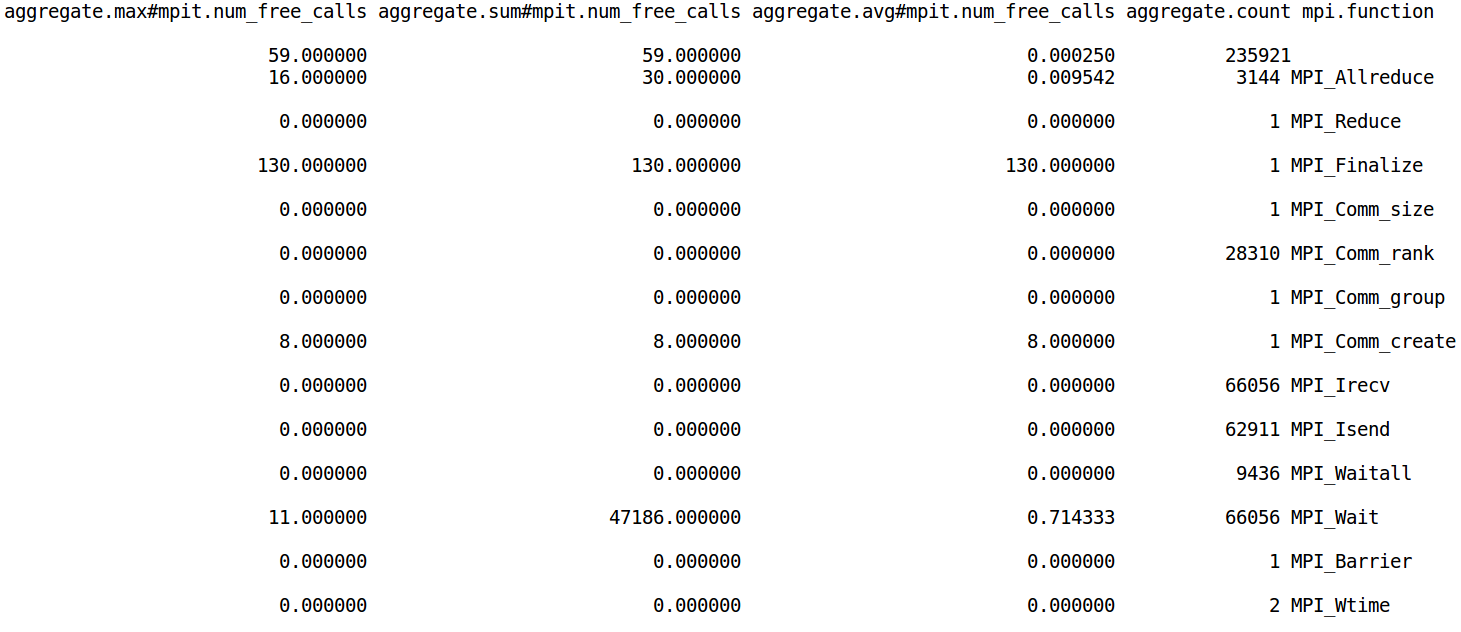
\includegraphics[scale=0.8, width=\columnwidth, height=3cm]{figures/CALIPER_MPI_counter_PVAR}
		\caption{PVAR aggregated across MPI routines}
		\label{fig:cali-counter}
	\end{figure*}
\end{center}
\par Although the two usage scenarios presented above are similar with respect to the set of services used, the MPI\_T sampling overheads involved vary significantly. I shall present these results in the following section.
\begin{center}
	\begin{figure*}[bp!]
         \centering
  \captionsetup{justification=centering}
		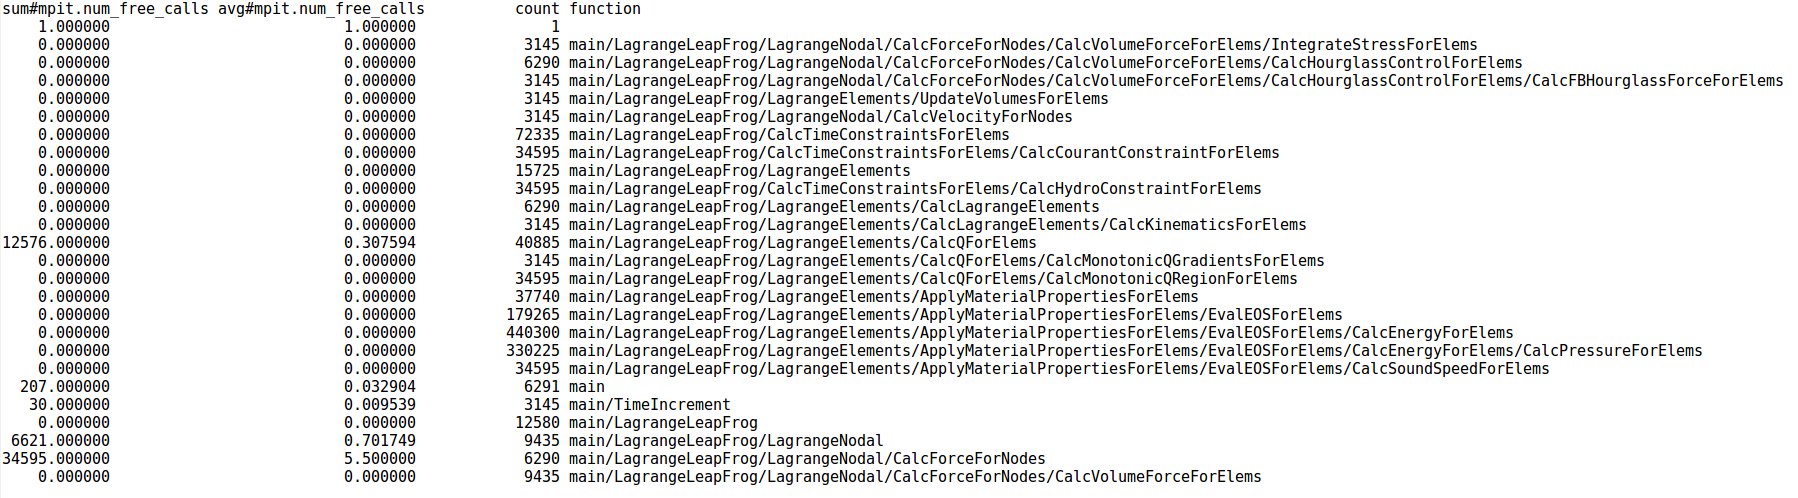
\includegraphics[scale=0.8, width=\columnwidth, keepaspectratio]{figures/CALIPER_app_counter_PVAR}
		\caption{PVAR aggregated across application routines}
		\label{fig:cali-app-counter}
	\end{figure*}
\end{center}

\section{Experiments}
In this section, I present results from a study focused on determining the sampling overheads for the MPI\_T support in Caliper.
\subsection{Experimental Setup}
All the experiments with LULESH were carried out on Quartz --- a 2600-node cluster at LLNL. Each node has two Intel Xeon E5-2695 18-core processors, providing a total of 36 cores and 128 GB of main memory. All our experiments were run using 27 MPI processes on one Quartz node --- a single node was sufficient for studying sampling overheads. In order to prevent performance variation between runs, the MPI processes were pinned to cores by setting \verb+MV2_ENABLE_AFFINITY+ to true. Each experiment was performed three times, and the runtime reported here is the averaged value. Two MVAPICH2 versions were used in this study --- MVAPICH2 version 2.3b and MVAPICH2 version 2.3rc2\footnote{http://mvapich.cse.ohio-state.edu/download/mvapich/mv2/mvapich2-2.3rc2.tar.gz}. 
\subsection{Results}
\subsubsection{Overhead in Enabling MPI\_T}
We first study how overheads vary when the number of PVARs exported by the MPI implementation differs. MVAPICH2 version 2.3b exports 73 PVARs, while MVAPICH2 version 2.3rc2 exports 402 PVARs. For this experiment, snapshots were triggered (and MPI\_T subsequently sampled for \textit{all} PVARs) whenever an MPI call was made. We define the following terms:
\begin{itemize}
\item \textbf{Baseline} --- Caliper-annotated LULESH profiled without any services enabled
\item \textbf{Without MPI\_T} --- Caliper-annotated LULESH profiled with the MPI, report, timestamp, aggregate, and event services enabled
\item \textbf{With MPI\_T} --- Caliper-annotated LULESH profiled with the MPI, MPI\_T, report, timestamp, aggregate, and event services enabled
\end{itemize}
Figure \ref{fig:cali-overhead-version} depicts an expected outcome --- the overheads are directly proportional to the number of PVARs exported. For MVAPICH2 version 2.3b, this corresponds to overheads of 76\% over the baseline, whereas for MVAPICH2 version 2.3rc2, overheads are 143\% over the corresponding baseline. None of these numbers are in an acceptable range --- this suggests that it is too expensive to sample \textit{all} PVARs, every time an MPI call is made.
\begin{center}
	\begin{figure*}[bp!]
         \centering
  \captionsetup{justification=centering}
		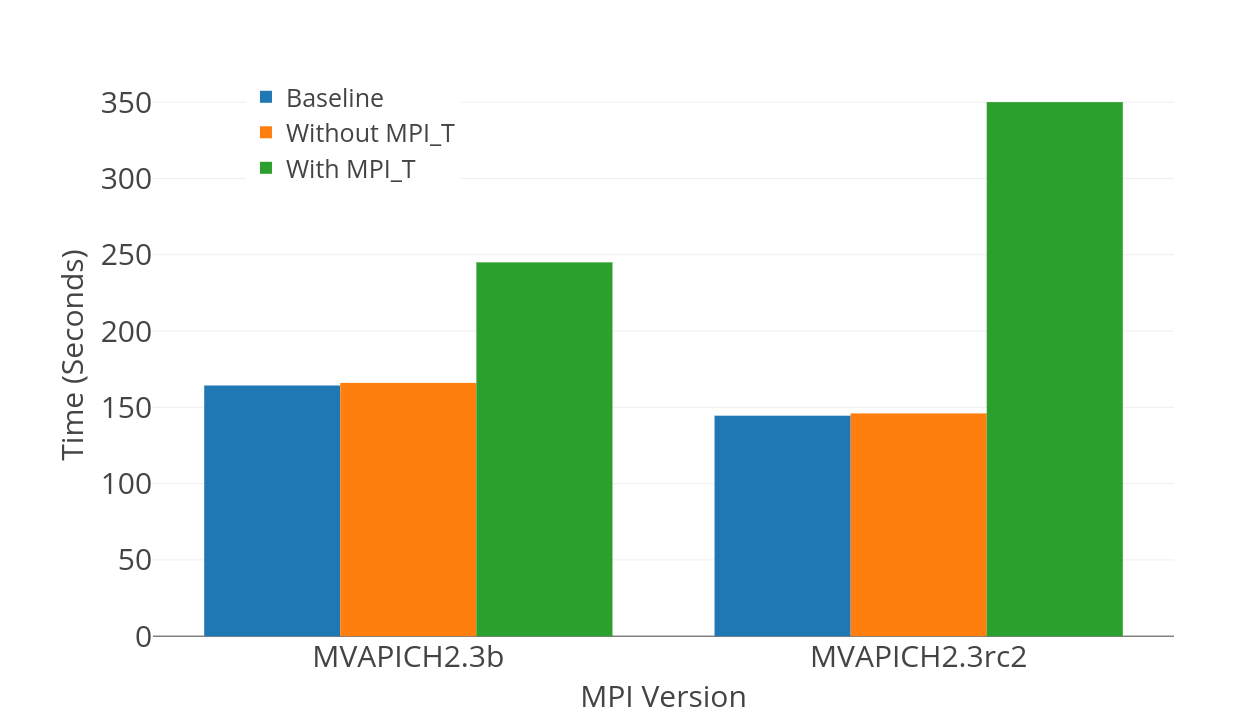
\includegraphics[scale=0.8, width=\columnwidth, keepaspectratio]{figures/CALIPER_overheads_version}
		\caption{LULESH: Variation of MPI\_T overhead with number of PVARs exported}
		\label{fig:cali-overhead-version}
	\end{figure*}
\end{center}

\par As alluded to in the section on usage scenarios, the snapshot-triggering mechanism has a significant impact on the MPI\_T sampling overheads. Specifically, we consider two situations:
\begin{itemize}
\item Snapshots triggered when an MPI call is made
\item Snapshots triggered when a Caliper-annotated application routine is invoked
\end{itemize}
For this experiment, the MVAPICH2 version 2.3rc2 was used. Figure \ref{fig:cali-overhead-snapshot} suggests that the overheads involved in triggering a snapshot and sampling MPI\_T from application-level routines are even higher than the situation where snapshots are triggered every time an MPI call is made. Specifically, we see overheads of 207\% when triggering snapshots from application-level routines, and overheads of 143\% when triggering snapshots from MPI routines. 
\par This is a sobering result --- even when the level of application instrumentation is low-to-moderate (such as in LULESH), MPI\_T sampling overheads are not acceptable. This would likely be the case in other scientific applications that are iterative (or depend on a timestep loop). A compromise solution in this situation may be to sample only a subset of PVARs --- perhaps by providing the user an environment variable to specify such a subset. But such a solution assumes that the user is already aware of the exact names (or indices) of the PVARs --- this is a poor assumption to make in the context of MPI\_T.
\begin{center}
	\begin{figure*}[bp!]
         \centering
  \captionsetup{justification=centering}
		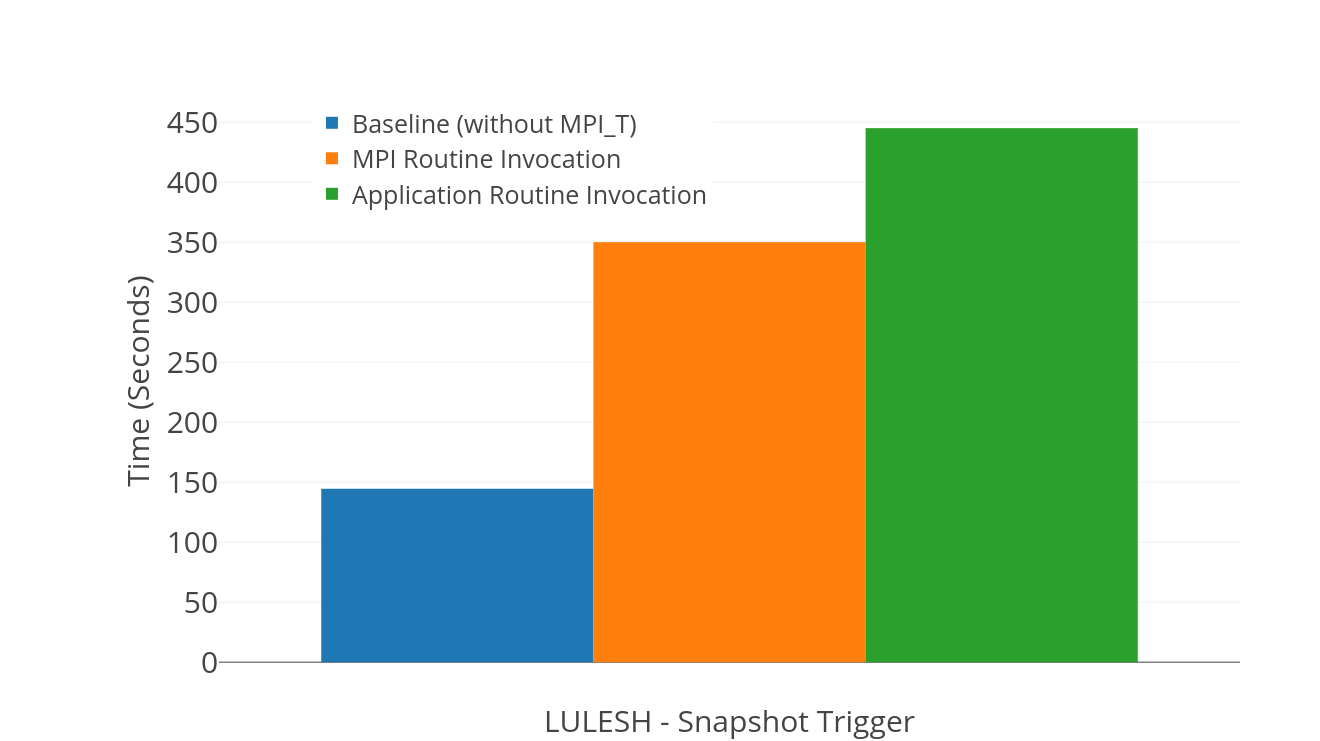
\includegraphics[scale=0.8, width=\columnwidth, keepaspectratio]{figures/CALIPER_overheads_snapshot_trigger}
		\caption{LULESH: Variation of MPI\_T overhead with snapshot trigger mechanism}
		\label{fig:cali-overhead-snapshot}
	\end{figure*}
\end{center}

\section{Implementation Challenges and Issues}
\subsection{Crashes with OpenMPI}
The MPI\_T support in Caliper was designed to be specifically used with the OpenMPI implementation. When this research was being carried out, OpenMPI was the only MPI library that had support for PVARs bound to MPI objects. However, we noted that the application crashed when we were trying to allocate handles for PVARs bound to MPI objects. This issue was communicated to the developers of the OpenMPI library. Unfortunately, this issue was not resolved in time, and we had to use MVAPICH2 for testing purposes.

\subsection{Lack of GUI support in Caliper}
When this research was being conducted, Caliper did not have GUI support for visualizing profiles, nor did it have support for writing out traces in a standard format. Caliper had basic text-based support for viewing and analyzing the collected performance data. Given the relatively large number of PVARs exported by MVAPICH2 (order of a 100), the basic text-based support was not sufficient to display all the data. We had to resort to viewing only a subset of PVARs at any given time.

\section{Bridge}
This chapter has described the design and implementation of the MPI\_T support in Caliper. Through experiments, we have demonstrated the capabilities and limitations of the performance introspection support in Caliper. In the next chapter, we shall present a discussion focusing on the design differences between the MPI\_T support in TAU and Caliper. 
